\chapter{Угловой момент}

\section{Повороты и оператор углового момента. Изотропность пространства и сохранение углового момента в квантовой механике.}

Переход от одной (1) декартовой системы координат (СК) к другой (2) повёрнутой СК всегда может быть осуществлён поворотом вокруг специально подобранного единичного вектора $\vec{n}$ на специально подобранный угол $\rchi$ (см.~\autoref{fig:8_1}).

\begin{figure}[h]
\centering
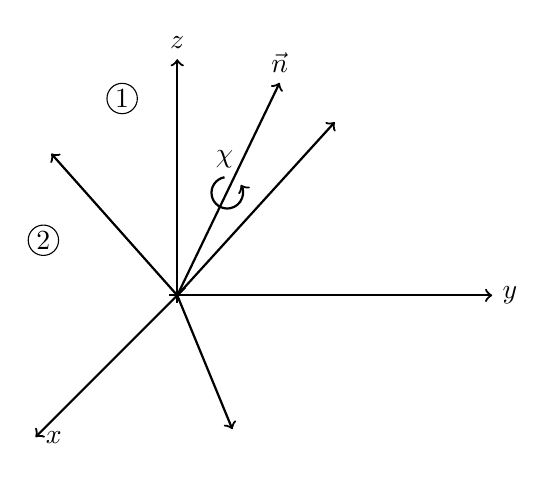
\begin{tikzpicture}[domain=-3:5]
  \draw[->, thick] (-0.1,0) -- (4,0) node[right] {$y$};
  \draw[->, thick] (0,-0.1) -- (0,3) node[above] {$z$};
  \draw[->, thick] (0.1,0.1) -- (-1.8,-1.8) node[right] {$x$};
  \draw (-0.7, 2.5) node[inner sep=1pt,draw,circle]  {$1$};
  \draw (-1.7, 0.7) node[inner sep=1pt,draw,circle]  {$2$};  
  \draw[->, thick] (0,0) -- (0.7,-1.7);
  \draw[->, thick] (0,0) -- (1.3,2.7) node[above] {$\vec n$};
  \draw[->, thick] (0,0) -- (2,2.2);
  \draw[->, thick] (0,0) -- (-1.6,1.8);
  \draw[->, thick] (0.6, 1.5) arc (-260:30:0.2cm);
  \node[above] at (0.6, 1.5) {$\chi$};
\end{tikzpicture}
\caption{Повороты в декартовой системе координат} \label{fig:8_1}
\end{figure}

Пусть $\rchi = \chi \vec{n}$ есть вектор поворота. Связь между векторами состояний системы в лабораториях 1 и 2 можно задать соотношением
$$
\ket{\psi;2} = \op{R}(\rchi) \ket{\psi;1}
$$%
%
где $\op{R}(\rchi)$ -- оператор поворота. Из сохранения нормировки векторов $\bk{\psi;2}{\psi;2} = \bk{\psi;1}{\psi;1}$ следует, что $\op{R}(\rchi)$ -- унитарный оператор. По аналогии с оператором эволюции (сдвига во времени) \eqref{eq:6_4_4} определим его в виде

\begin{equation}
\label{eq:8_1_1}
\boxed {
	\op{R}(\op{\rchi}) \equiv e^{-(i/\hbar) \opv{J} \rchi}
}
\end{equation}
где $\opv{J}$ -- некоторый векторный эрмитовый оператор, не зависящий от времени.

Из изотропности пространства следует, что если $\ket{\psi;1}$ удовлетворяет уравнению Шрёдингера, то и $\ket{\psi;2}$ также является решением уравнения Шрёдингера:

$$
i\hbar \pd{\ket{\psi;2}}{t} = i\hbar \op{R}(\rchi) \pd{\ket{\psi;1}}{t} = \op{R}(\rchi) \op{H}\ket{\psi;1}
$$%
%
С другой стороны:
$$
i\hbar \pd{\ket{\psi;2}}{t} = \op{H}\ket{\psi;2} = \op{H} \op{R}(\rchi) \ket{\psi;1}
$$%
%
Заметим, что согласно определению \eqref{eq:8_1_1} $\op{R}(\rchi)$ представляет собой ряд по степеням оператора $\opv{J}$

$$
\op{R}(\rchi) = \sum_{k=0}^{\infty} \frac{1}{k!} \brc{- \frac{i}{\hbar} \opv{J} \rchi}^k
$$%
%
поэтому из коммутативности $\brs{\op{H}, \op{R}(\rchi)} = 0$ следует коммутативность

\begin{equation}
\label{eq:8_1_2}
\boxed {
	\brs{\op{H}, \opv{J}} = 0
}
\end{equation}

\begin{excr}
Доказать \eqref{eq:8_1_2}
\end{excr}

Таким образом, условие изотропность пространства приводит нас к сохраняющейся векторной величине $\vec{J}$, отвечающей оператору $\opv{J}$, т.е. к интегралу движения $\vec{J}$. В классической механике величиной, сохраняющейся во времени вследствие изотропность пространства, является угловой момент (см.~\llref{9}{1}, <<Сохранение углового момента>>). Поэтому естественно принять, что $\opv{J}$ есть {\em оператор углового момента}. В квантовой механике термин {\em угловой момент } представляет обобщающее понятие. Он включает в себя операторы $\opv{L}$ -- орбитального, $\opv{S}$ -- спинового, и $\opv{J} = (\opv{L} + \opv{S})$ -- полного момента квантовой частицы.

\begin{sloppypar}
  \section{Коммутационные соотношения для оператора углового момента. Система собственных векторов операторов \texorpdfstring{$\opv{j}^2$ и $\opv{j}_z$}{углового момента}}
\end{sloppypar}

Введём безразмерный оператор углового момента
$$
\boxed{
  \opv{j} = \frac{\opv{J}}{\hbar}
}
$$

\begin{defn}
Векторный оператор $\opv{j} = \brcr{\op{j_x}, \op{j_y}, \op{j_z}}$ называют \underline{оператором углового момента}, если все его компоненты являются наблюдаемыми (эрмитовыми) и удовлетворяют коммутационным соотношениям:
\begin{equation}
\label{eq:8_2_1}
\boxed {
	\brs{\op{j_i}, \op{j_k}} = i e_{ikl} \op{j_l}
}
\end{equation}
\end{defn}
%
Здесь $e_{ikl}$ -- антисимметричный единичный тензор третьего ранда, по дважды повторяющимся индексам подразумевается суммирование.

Оператор квадрата углового момента связан с операторами проекции на координатные оси следующим образом
$$
\opv{j}^2 = \op{j_x}^2 + \op{j_y}^2 + \op{j_z}^2
$$%
%
Пользуясь  коммутационными соотношениями \eqref{eq:8_2_1}, нетрудно доказать, что для всех $i=x, y, z$
\begin{equation}
\label{eq:8_2_2}
\brs{\opv{j}^2, \op{j_i}} = 0
\end{equation}

\begin{excr}
Доказать \eqref{eq:8_2_2} с помощью \eqref{eq:8_2_1}
\end{excr}

Таким образом, в квантовой механике совместно измеримы квадрат углового момента и только одна из его компонент -- любая на выбор! Традиционно полагают, что это $\op{j}_z$.

Пусть $\ket{jm}$ образуют систему собственных векторов $\opv{j}^2$ и  $\op{j}_z$ с собственными значениями $\lambda(j)$ и $m$:

\begin{equation}
\label{eq:8_2_3}
\left\{
\begin{aligned}
\opv{j}^2 \ket{jm} = \lambda(j) \ket{jm} \\
\op{j}_z \ket{jm} = m \ket{jm}
\end{aligned}
\right.
\end{equation}%
%
Эти собственные векторы ортонормированы
$$
\bk{jm}{j'm'} = \delta_{jj'} \delta_{mm'}
$$%
%
По физическому смыслу $m$ -- это проекция вектора $\vec{j}$ на ось $0z$, $\lambda(j)$ -- квадрат длины вектора углового момента. Попробуем разобраться, какие значения могут принимать $\lambda(j)$ и $m$, пользуясь только коммутационными соотношениями.

Прежде всего заметим, что т.е. в любом состоянии
$$
\avg{\opv{j}^2} = \avg{\op{j_x}^2} + \avg{\op{j_y}^2} + \avg{\op{j_z}^2} \geqslant \avg{\op{j_z}^2}
$$%
%
то $\lambda(j) \geqslant m^2$, а это значим, что само $m$ ограничено сверху и снизу
$$
m_{min} \leqslant m \leqslant m_{max}
$$%
%
Очевидно, что $m_{max} = - m_{min}$. Пусть $m_{max} \equiv j$ (верхняя граница изменения проекции вектора $\vec{j}$ на ось $0z$ лимитирована его модулем), тогда $m_{min} = -j$.

Введём операторы:
\begin{equation}
\label{eq:8_2_4}
\left\{
\begin{aligned}
\op{j}_{+} &= \op{j}_{x} + i \op{j}_{y} \\
\op{j}_{-} &= \op{j}_{x} - i \op{j}_{y} = \brc{\op{j}_{+}}^\dag
\end{aligned}
\right.
\end{equation}%
%
Они не эрмитовы, но эрмитово сопряжены друг другу и удовлетворяют коммутационным соотношениям
\begin{equation}
\label{eq:8_2_5}
\brs{\op{j_z}, \op{j}_{\pm}} = \pm \op{j_{\pm}}
\end{equation}%
%
\begin{excr}
Доказать \eqref{eq:8_2_5} с использованием \eqref{eq:8_2_4} и \eqref{eq:8_2_1}
\end{excr}

Операторы $\op{j}_{\pm}$ имеют определённую аналогию с $\cre$ и $\ann$ в теории гармонического осциллятора. Действительно
$$
\left. \op{j_z} \brc{\op{j}_{\pm} \ket{jm}} \right|_{\text{\eqref{eq:8_2_5}}}
= \left. \brc{\op{j}_{\pm} \op{j_z} \pm \op{j}_{\pm}} \ket{jm} \right|_{\text{\eqref{eq:8_2_3}}}
= (m \pm 1) \brc{\op{j}_{\pm} \ket{jm}}
$$%
%
т.е. $\op{j}_{\pm} \ket{jm}$ -- тоже собственные векторы операторов $\opv{j}^2$ и $\op{j}_z$, отвечающие собственным значениям $\lambda(j)$ (для $\opv{j}^2$) и $m \pm 1$ (для $\op{j}_z$). Следовательно, $\op{j}_{+}$ и $\op{j}_{-}$ -- операторы {\em повышения} и {\em понижения} соответственно, поэтому

\begin{equation}
\label{eq:8_2_6}
\left\{
\begin{aligned}
\op{j}_{+} \ket{j, m-1} &= \alpha_m \ket{j, m}\\
\op{j}_{-} \ket{j, m} &= \beta_m \ket{j, m-1}\\
\end{aligned}
\right.
\end{equation}%
%
Поскольку спектр значений $m$ ограничен сверху, то $\op{j}_{+} \ket{jj} = 0$ (или $\alpha_{j+1} = 0$), а также ограничен снизу, то $\op{j}_{-} \ket{j, -j} = 0$ (или $\beta_{-j} = 0$).

Воспользовавшись оператором понижения, запишем
$$
\left\downarrow
\begin{aligned}
\op{j}_{-} \ket{jj} & \sim \ket{j, j-1}\\
(\op{j}_{-})^2 \ket{jj} & \sim \ket{j, j-2}\\
\cdots \\
(\op{j}_{-})^N \ket{jj} & \sim \ket{j, j-N},~~~N \in \mathbb{N} \cup \brcr{0} \\
\end{aligned}
\right.
$$%
%
Предположим, что каким-то образом мы осуществляем переход от состояния с максимальной проекцией $\ket{jj}$ к состоянию с минимальной проекцией $\ket{j, -j}$. Тогда $j - N = -j$, т.е. $j = N/2$. Таким образом, $j$ может принимать либо целые, либо полуцелые значения:
$$
j = 0, \frac{1}{2}, 1, \frac{3}{2} \cdots
$$%
%
При фиксированном $j$ существуют следующие проекции углового момента:
$$
m = \underbrace{-j, -j + 1, \cdots, j}_{(2j + 1)~\text{значения}}
$$%
%
т.е. всего существует $(2j+1)$ состояний $\ket{jm}$ при определённом угловом моменте $j$. Величина $j$ обычно называется {\em квантовым числом момента количества движения частицы}, а $m$ -- {\em магнитным квантовым числом}.

Найдём теперь все $\lambda(j)$. Поскольку $\lambda(j)$ не зависит от $m$, то положим $m_{max} = -m_{min} \equiv j$. Тогда
$$
\op{j}_{-} \op{j}_{+} \ket{jj} = 0
$$%
%
\begin{excr}
Доказать
$$
\op{j}_{-} \op{j}_{+} = \opv{j}^2 - \op{j_z}^2 - \op{j_z}
$$
используя \eqref{eq:8_2_4} и \eqref{eq:8_2_1}
\end{excr}%
%
Используя равенство из упражнения, получаем
$$
\brc{\opv{j}^2 - \op{j_z}^2 - \op{j_z}} \ket{jj} = 0 ~~~~~~ \lambda(j) = j(j+1)
$$
\begin{equation}
\label{eq:8_2_7}
\boxed {
	\opv{j}^2 \ket{jm} = j(j+1) \ket{jm}
}
\end{equation}

Вычислим $\alpha_m$ и $\beta_m$ в \eqref{eq:8_2_6}. Заметим, что
$$
\begin{gathered}
\alpha_m = \bfk{jm}{\op{j}_{+}}{j, m-1} = \bk{\op{j}_{-}jm}{j, m-1} =\\= \left. \bfk{j,m-1}{\op{j}_{-}}{jm}^* \right|_{\text{\eqref{eq:8_2_6}}} = \beta_m^*
\end{gathered}
$$%
%
т.е. требуется определить следующие ненулевые коэффициенты:
$$
\beta_{-j+1}, \beta_{-j+2}, \cdots, \beta_{j}
$$%
%
Имеем, с одной стороны,
$$
\left. \op{j}_{+} \op{j}_{-} \ket{jm} \right|_{\text{\eqref{eq:8_2_6}}}
= \left. \beta_m \op{j}_{+} \ket{j, m-1} 
= \right|_{\text{\eqref{eq:8_2_6}}} \abs{\beta_m}^2 \ket{jm}
$$%
%
с другой стороны:
$$
\op{j}_{+} \op{j}_{-} = \opv{j}^2 - \op{j_z}^2 + \op{j_z}
$$

\begin{excr}
Доказать предыдущее равенство используя \eqref{eq:8_2_4} и \eqref{eq:8_2_1}
\end{excr}%
%
\noindent
Также имеем:
$$
\op{j}_{+} \op{j}_{-} \ket{jm} = \left. (\opv{j}^2 - \op{j_z}^2 + \op{j_z}) \ket{jm} \right|_{\text{\eqref{eq:8_2_7}, \eqref{eq:8_2_3}}} = \brc{j(j+1) - m^2 + m} \ket{jm}
$$%
%
Выберем в \eqref{eq:8_2_6} фазы векторов состояний $\ket{jm}$ так, чтобы $\alpha_m = \beta_m$ были действительными неотрицательным числами. Тогда
$$
\beta_m = \sqrt{j^2 + j - m^2 + m} = \sqrt{(j+m)(j-m+1)} = \alpha_m
$$%
%
то есть
$$
\begin{gathered}
\op{j}_{-} \ket{jm} = \sqrt{(j+m)(j-m+1)} \ket{j, m-1} \\
\op{j}_{+} \ket{jm} = \beta_{m+1} \ket{j, m+1} = \sqrt{(j-m)(j+m+1)} \ket{j, m+1}
\end{gathered}
$$

\begin{equation}
\label{eq:8_2_8}
\boxed {
	(\op{j_x} \pm i \op{j_y}) \ket{jm} = \sqrt{(j \mp m)(j \pm m + 1)} \ket{j, m \pm 1}
}
\end{equation}


\section{Спин частицы. Матрицы Паули.}

Собственный угловой момент частицы называют {\em спиновым моментом}, или просто {\em спином}. Спин обычно обозначают буквой $s$, $\opv{s} = \brcr{\op{s}_x, \op{s}_y, \op{s}_z}$ -- оператор спина.

Рассмотрим частицу со спином $s = 1/2$. Согласно общей теории углового момента, базисные векторы $\ket{s, m_s}$, где $s = 1/2$, являются собственными векторами операторов $\opv{s}^2$ и $\op{s}_z$:

\begin{equation}
\label{eq:8_3_1}
\left\{
\begin{array}{l}
\opv{s}^2 \ket{s m_s} = s(s+1) \ket{s m_s}\\
\op{s}_z \ket{s m_s} = m_s \ket{s m_s}
\end{array}
\right.
\end{equation}%
%
При $s=1/2$ проекция спина на выделенное направление, например, на ось $Z$, может принимать $2s + 1 = 2$ значения: $m_s = \pm 1/2$. Базисные векторы этого представления $\chi_{1/2, m_s} \equiv \ket{1/2, m_s}$ имеют вид

\begin{equation}
\label{eq:8_3_2}
  \begin{array}{l}
  \chi_{\frac{1}{2}, \frac{1}{2}} \equiv \ket{\frac{1}{2}, \frac{1}{2}} \equiv \begin{pmatrix} 1 \\ 0 \end{pmatrix}    \equiv \ket{\alpha} \equiv \ket{+}\\
  \chi_{\frac{1}{2}, -\frac{1}{2}} \equiv \ket{\frac{1}{2}, -\frac{1}{2}} \equiv \begin{pmatrix} 0 \\ 1 \end{pmatrix}   \equiv \ket{\beta} \equiv \ket{-}
\end{array}
\end{equation}%
%
Векторы $\ket{\frac{1}{2}, \frac{1}{2}}$ и $\ket{\frac{1}{2}, -\frac{1}{2}}$ образуют полный ортонормированный базис в пространстве спиновых состояний частицы, поэтому произвольное спиновое состояние частицы со спином $s=1/2$ можно представить в виде разложения по собственным векторам \eqref{eq:8_3_2} оператора $\op{s}_z$

\begin{equation}
\label{eq:8_3_3}
\boxed{
	\ket{\chi} = a_{+} \begin{pmatrix} 1 \\ 0 \end{pmatrix} + a_{-} \begin{pmatrix} 0 \\ 1 \end{pmatrix} = \begin{pmatrix} a_{+} \\ a_{-} \end{pmatrix}
}
\end{equation}%
%
Из условия нормировки $\avg{\chi, \chi} = 1$ следует, что 
$$
\abs{a_{+}}^2 + \abs{a_{-}}^2 = 1
$$%
%
Поэтому удобно изобразить векторы состояния частицы со спинами $s=1/2$ в виде двухкомпонентного столбца \eqref{eq:8_3_3} или {\em спинора}, где в соответствии с вероятностной интерпретацией квантовой механики, верхняя компонента есть амплитуда вероятность найти частицу в состоянии с $s_z = +1/2$, а нажняя -- в состоянии с $s_z = -1/2$. Точно также волновую функцию частицы с любым спином $s$ можно записать (2s+1)-компонентным столбцом.

В собственном представлении \eqref{eq:8_3_1} матрицы операторов $\opv{s}^2$ и $\op{s}_z$ диагональны, и диагональные элементы равны их собственным значениям (см.~\sref{1}{6}):
\begin{equation}
\label{eq:8_3_4}
\opv{s}^2 = \frac{3}{4}
\begin{matrix}
            & \ket{+} & \ket{-} \\
\bra{+} &  1         & 0         \\
\bra{-}  &  0         & 1         
\end{matrix}
~~~\op{s}_z = \frac{1}{2}
\begin{matrix}
            & \ket{+} & \ket{-} \\
\bra{+} &  1         & 0         \\
\bra{-}  &  0         & -1         
\end{matrix}
\end{equation}%
% TODO: отрисовать получше
%
Легко проверить, что векторы \eqref{eq:8_3_2}, как и должно быть, являются собственными векторами матрицы $\op{s}_z$ с собственными значениями $\pm 1/2$.

Введём теперь повышающий и понижающий операторы
$$
\op{s}_{\pm} = \op{s}_x \pm i\op{s}_y
$$%
%
для спина $s=1/2$, которые действуют на состояния \eqref{eq:8_3_2}, согласно общим соотношениями \eqref{eq:8_2_8}, следующим образом
$$
\begin{matrix}
\op{s}_{+}\ket{+} = 0 & \op{s}_{+}\ket{-} = \ket{+} \\
\op{s}_{-}\ket{-} = 0 &  \op{s}_{-}\ket{+} = \ket{-}
\end{matrix}
$$%
%
Матрицы операторов $\op{s}_{+}$ и $\op{s}_{-}$ имеют вид

\begin{equation}
\label{eq:8_3_5}
\op{s}_{+} = 
\begin{matrix}
            & \ket{+} & \ket{-} \\
\bra{+} &  0         & 1         \\
\bra{-}  &  0         & 0         
\end{matrix}
~~~~~\op{s}_{-} = (\op{s}_{+})^\dag = 
\begin{matrix}
            & \ket{+} & \ket{-} \\
\bra{+} &  0         & 0         \\
\bra{-}  &  1         & 0         
\end{matrix}
\end{equation}%
%
Наконец, переходя от $\op{s}_{\pm}$ к $\op{s}_x$ и $\op{s}_y$, находим

\begin{equation}
\label{eq:8_3_6}
\begin{gathered}
\op{s}_x = \frac{\op{s}_{+} + \op{s}_{-}}{2} = \frac{1}{2} \left (
  \begin{matrix}
  0 & 1 \\
  1 & 0 
  \end{matrix}
\right )
\\
\op{s}_y = \frac{\op{s}_{+} - \op{s}_{-}}{2i} = \frac{1}{2} \left (
  \begin{matrix}
  0 & -i \\
  i & 0 
  \end{matrix}
\right )
\end{gathered}
\end{equation}

Матрицы \eqref{eq:8_3_4} и \eqref{eq:8_3_6} операторов спина $\opv{s} = \brcr{\op{s}_x, \op{s}_y, \op{s}_z}$ обычно выражают через {\em матрицы Паули} $\opv{\sigma} = \brcr{\op{\sigma}_x, \op{\sigma}_y, \op{\sigma}_z}$, вводя соответствующие $\sigma$-операторы

$$
\boxed{
\begin{gathered}
  \opv{s}= \frac{1}{2}\msigm\\
  \op{\sigma}_x = \left (
    \begin{matrix}
    0 & 1 \\
    1 & 0 
    \end{matrix}
  \right )
  ~~~
  \op{\sigma}_y = \left (
    \begin{matrix}
    0 & -i \\
    i & 0 
    \end{matrix}
  \right )
  ~~~
  \op{\sigma}_z = \left (
    \begin{matrix}
    1 & 0 \\
    0 & -1 
    \end{matrix}
  \right)
\end{gathered}
}
$$%
%
С алгеброй матриц Паули можно познакомиться, решив \cref{ex:1_2_6}, \cref{ex:1_2_7} и задачу 4 из 2-го задания.

\section{Оператор орбитального момента частицы в координатном представлении (декартовы и сферические координаты)}

В классическом механике {\em момент количества движения частицы} (или {\em орбитальный момент}) определяется как векторное произведение радиус-вектора $\vr$ частицы и её импульса $vp$ (см.~\llref{9}{1})
$$
\vec{L} = \vr \times \vp
$$%
%
В квантовой механике, согласно принципу соответствия (см.~\sref{2}{5}), физической величине $\vec{L}$ сопоставляется оператор
\begin{equation}
\label{eq:8_4_1}
\boxed{
  \opv{L} = \hbar \opv{l} = \op{\vr} \times \op{\vp}
}
\end{equation}%
%
Его реализацией в координатном представлении будет
\begin{equation}
\label{eq:8_4_2}
  \opv{L} = \hbar \opv{l} \equiv -i\hbar(\vr \times \nabla)
\end{equation}%
%
ибо $\opv{p} = -i\hbar\nabla$. По определению
$$
\opv{l} = \frac{\op{\vec L}}{\hbar} = -i(\vr \times \nabla) = -i \left| 
  \begin{matrix}
  \vec{i} & \vec{j} & \vec{k}\\
  x & y & z\\
  \pd{}{x} & \pd{}{y} & \pd{}{z}\\
  \end{matrix}
  \right |
$$%
%
есть {\em безразмерный оператор орбитального момента} $\op{\vec l} = \brcr{\vec{l}_x, \vec{l}_y, \vec{l}_z}$, где, например,
$$
  \vec{l}_z = -i \brc{x \pd{}{y} - y \pd{}{x}}
$$%
%
или в общем виде
\begin{equation}
\label{eq:8_4_3}
  \vec{l}_\alpha = -i e_{\alpha \beta \gamma} x_\beta \pd{}{x_\gamma},~\alpha, \beta, \gamma = 1, 2, 3
\end{equation}

Если воспользоваться определением операторов проекций момента в тензорных обозначениях \eqref{eq:8_4_3}, то можно убедиться в справедливости коммутационных соотношений \eqref{eq:8_2_1} для углового момента
\begin{equation}
\label{eq:8_4_4}
  [\op{l}_\alpha, \op{l}_\beta] = i e_{\alpha \beta \gamma} \op{l}_\gamma
\end{equation}%
%
Для оператора квадрата орбитального момента
$$
\opv{l}^2 = \op{l}^2_x + \op{l}^2_y + \op{l}^2_z
$$%
%
пользуясь \eqref{eq:8_4_4}, нетрудно показать, что он коммутирует с операторами проекций, т.е.
\begin{equation}
\label{eq:8_4_5}
  \boxed{[\opv{l}^2, \op{l}_\alpha] = 0}.
\end{equation}%
%
(см.~соотношения \eqref{eq:8_2_2} в теории углового момента).

\begin{figure}[h]
\centering
\begin{tikzpicture}[domain=-3:5]
  \draw[->, thick] (-0.1,0) -- (4,0) node[right] {$y$};
  \draw[->, thick] (0,-0.1) -- (0,3) node[above] {$z$};
  \draw[->, thick] (0.1,0.1) -- (-1.8,-1.8) node[right] {$x$};
  \draw[->] (0, 0) -- (1,-1);
  \draw[dashed] (2, 0) -- (1,-1);  
  \draw[dashed] (-1, -1) -- (1,-1);   
  \draw[->] (0, 0) -- (1,2.5) node[above] {r};
  \draw[dashed] (0, 2.8) -- (1, 2.5);
  \draw[dashed] (1, 2.5) -- (1, -1);
  \draw[-] (-0.4, -0.4) arc (-135:-45:0.57cm);
  \node[above] at (0, -1.1) {$\psi$};
  \draw[-] (0, 0.7) arc (90:65:0.7cm);
  \node[left] at (0.4, 1) {$\theta$};

\end{tikzpicture}
\caption{Сферическая система координат} \label{fig:8_2}
\end{figure}

Перейдём от декартовых координат $(x,y,z)$ к сферическим координатам $(r, \theta, \phi)$:

$$
\begin{gathered}
\begin{cases}
x = r \sin \theta \cos \phi \\
y = r \sin \theta \sin \phi \\
z = r \cos \theta
\end{cases}\\
0 \le r \le \infty,~~~0 \le \theta \le \pi, ~~~ 0 \le \phi \le 2\pi
\end{gathered}
$$%
%
Затем следует провести преобразование координат по схеме
$$
\pd{}{\phi} =\underbrace{\pd{x}{\phi}}_{\mathclap{-r \sin \theta \sin \phi}} \cdot \pd{}{x} + \underbrace{\pd{y}{\phi}}_{\mathclap{r \sin \theta \cos \phi}}\cdot \pd{}{y} + \cancel{\pd{z}{\phi} \cdot \pd{}{z}} =
x \pd{}{y} - y \pd{}{x}
$$%
%
отсюда
$$
\boxed{\op{l}_z = -i \pd{}{\phi}}
$$%
%
Таким же образом переходят в сферических координатах для
$$
\begin{gathered}
\op{l}_x = -i(-\sin \phi \pd{}{\theta} - \cos \phi \ctg \theta \pd{}{\phi})\\
\op{l}_y = -i(\cos \phi \pd{}{\theta} - \sin \phi \ctg \theta \pd{}{\phi})
\end{gathered}
$$%
%
Для оператора квадрата орбитального момента:
$$
\opv{l}^2 = -\brs{ \frac{1}{\sin \theta} \pd{}{\theta} \brc{\sin \theta \pd{}{\theta}} + \frac{1}{\sin \theta} \pd{^2}{\phi^2}} = - \Delta_{\theta, \phi}
$$%
%
Здесь $\Delta_{\theta, \phi}$ определяет {\em угловую часть} лапласиана в сферических координатах
$$
\Delta_{\vr} = \underbrace{\frac{1}{r^2} \pd{}{r} \brc{r^2 \pd{}{r}}}_{\Delta_r,~\text{радиальная часть}} + \underbrace{ \frac{1}{r^2} \Delta_{\theta, \phi}}_{\text{угловая часть}}
$$%
%
поэтому оператор Гамильтона можно записать как
\begin{equation}
\label{eq:8_4_6}
\op{H} = - \frac{\hbar^2}{2m} \brc{\frac{1}{r^2} \pd{}{r} \brc{r^2 \pd{}{r}} - \frac{\vec{l}^2}{r^2}} + U(\vr)
\end{equation}

\section{Сферические гармоники}

В координатном представлении уравнение на собственные значения и собственные функции оператора $\op{l}_z = -i \pd{}{\phi}$ имеет вид
\begin{equation}
\label{eq:8_5_1}
-i \pd{}{\phi} \underbrace{\bk{\phi}{m}}_{\equiv~\Phi_m(\phi)} = m \bk{\phi}{m}
\end{equation}%
%
где $\Phi_m(\phi)$ -- $m$-я собственная функция оператора $\op{l}_z$. решением уравнения $\eqref{eq:8_5_1}$ является
\begin{equation}
\label{eq:8_5_2}
  \Phi_m(\phi) = C e^{i m \phi}
\end{equation}%
%
где $C$ -- нормировочная постоянная. При изменении угла $\phi$ на $2\pi$ мы возвращаемся в исходную точку пространства. Поскольку волновая функция должна быть однозначной, то
$$
\begin{gathered}
\Phi_m(\phi) = \Phi_m(\phi + 2\pi) \\
e^{im2\pi} = 1
\end{gathered}
$$%
%
В результате реализуется целочисленный вариант квантования проекции орбитального момента: $m=0, \pm 1, \pm 2, ...$. При $C = 1/\sqrt{2\pi}$ собственные функции нормированы условием
$$
\int_0^{2\pi} \diff\phi \Phi^*_m(\phi) \Phi_{m'}(\phi) = \delta_{mm'} 
$$

Общие собственные векторы операторов $\opv{l}^2$ и $\op{l}_z$, согласно теории углового момента, удовлетворяют системе уравнений
\begin{equation}
\label{eq:8_5_3}
\left\{
  \begin{matrix}
    \opv{l}^2 \ket{lm} = l(l+1)\ket{lm} \\
    \op{l}_z \ket{lm} = m \ket{lm}
  \end{matrix}
\right.
\end{equation}%
%
Решениями этой системы в сферических координатах
\begin{equation}
\left\{
  \begin{matrix}
  \label{eq:8_5_3_add}
   - \Delta_{\theta, \phi} Y_{lm}(\theta, \phi) = l(l+1) Y_{lm}(\theta, \phi) 
    \\
     -i\pd{}{\phi} Y_{lm}(\theta, \phi) = m Y_{lm}(\theta, \phi) 
  \end{matrix}
\right .
\tag{\ref{eq:8_5_3}$'$}
\end{equation}%
%
являются {\em сферические функции} или {сферические гармоники} $Y_{lm}(\theta, \phi) \equiv \bk{\theta, \phi}{lm}$. Их можно представить в виде
$$
Y_{lm}(\theta, \phi) = \Theta_{lm}(\theta) \Phi_m(\phi)
$$%
%
как результат решения системы дифференциальных уравнений \eqref{eq:8_5_3_add} методом разделения переменных. После <<отделения>> уравнения для $\Phi_m(\phi)$ (с условием однозначности $\Phi_m(\phi) = \Phi_m(\phi + 2\pi)$) остаётся уравнения для $\Theta_{lm}(\theta)$ с дополнительным условием $\abs{\Theta_{lm}(\theta)}_{[0,\pi]} < \infty$. Чтобы у функции $\Theta_{lm}(\theta)$ не было особенностей в точках $0$ и $\pi$, решение должно представлять собой полином, а конкретно
$$
\boxed{
  Y_{lm}(\theta, \phi) = C_{lm} e^{im\phi} P^m_l(\cos \theta)
}
$$%
%
где  $P^m_l(\cos \theta)$ -- присоединенные полиномы Лежандра. Здесь квантовые числа $l = \abs{m}, \abs{m} + 1, \dots, (l \ge \abs{m})$, т.е. при целочисленных $l = 0, 1, 2, ...$ имеем $m = 0, \pm 1, \pm 2, ..., \pm l$.

Отметим, что в спектроскопии используются специальные обозначения для орбитального квантового числа $l$:
$$
\begin{matrix}
l =  & 0 & 1 & 2 & 3 & ... & \\
       & s & p & d & f & ... & \text{-- состояния}
\end{matrix}
$$%
%
Сферические гармоники образуют полный ортонормированный базис на сфере единичного радиуса $(r = 1,~0 \leqslant \theta \leqslant \pi,~0 \leqslant \phi \leqslant 2\pi)$
\begin{equation}
\label{eq:8_5_4}
\boxed{\bk{Y_{lm}}{Y_{l'm'}} = \int_0^{2\pi} \diff\phi \int_0^\pi \sin \theta \diff\theta Y^*_{lm}(\theta, \phi) Y_{l'm'}(\theta, \phi) = \delta_{ll'} \delta_{mm'}}
\end{equation}